\documentclass[10pt,a4paper]{beamer}
\usepackage[utf8]{inputenc}
\usepackage[spanish]{babel}
\usepackage{amsmath}
\usepackage{amsfonts}
\usepackage{amssymb}
\usepackage{makeidx}
\usepackage{graphicx}
\author{Clinton Semanate}
\begin{document}


\begin{frame}{Ejercicio Resuelto\\
}{Fuente: Ecuaciones Diferenciales-Deniss Zill, Cap. 11, Vol. 1, Pág. 545.
Cálculo de la temperatura u en una placa rectangular}

\begin{center}
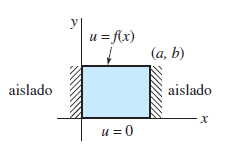
\includegraphics[scale=0.7]{placa.png} 
\end{center}

  \begin{itemize}
  \item
    Suponga que deseamos encontrar la temperatura de estado estable
$u(x, y)$ en una placa rectangular cuyas orillas verticales $x=0 x=a$ se encuentran aisladas,
mientras las orillas superior e inferior $y=b y=0$ se mantienen a temperaturas f (x)
y 0, respectivamente. Consulte la figura cuando no escapa calor desde las superficies
laterales de la placa, resolvemos el siguiente problema de valores en la frontera:\\
$\dfrac{d^{2}u}{dx^{2}}+\dfrac{d^{2}u}{dy^{2}}=0, $
$ 0<x<a,$
$0<y<b,$ (1)\\

  \end{itemize}
\end{frame}

\begin{frame}{Ejercicio Resuelto\\
}{Fuente: Ecuaciones Diferenciales-Deniss Zill, Cap. 11, Vol. 1, Pág. 545.
Cálculo de la temperatura u en una placa rectangular}


  \begin{itemize}
  \item
    $\dfrac{du}{dx}|x=0 =0, $ 
$ \dfrac{du}{dx}|x=a =0, $ $ 0<y<b,$ (2)\\
$u(x,0)=0 ,  u(x,b)=f(x), $ $0<x<a,$ (3)\\
Solución del problema de valores en la frontera.\\
Con $u(x,y)=X(x)Y(y),$ la separación de variables en (1) conduce a\\
$$\dfrac{X^{"}}{X}=-Y^{"}{Y}=-\lambda$$\\
$X^{"}+\lambda.X=0,$ (4) \\
$Y^{"}+\lambda.Y=0,$ (5)\\
    
  \end{itemize}
\end{frame}

\begin{frame}{Ejercicio Resuelto\\
}{Fuente: Ecuaciones Diferenciales-Deniss Zill, Cap. 11, Vol. 1, Pág. 545.
Cálculo de la temperatura u en una placa rectangular}


  \begin{itemize}
  \item
    En (2) y (3), las tres condiciones de frontera homogéneas se traducen en $X^{'}(0)=0$, $X^{'}(a)=0$ y $Y(0)=0$. El problema de Sturm-Liouville asociado con la ecuación (4) es entonces\\
$X^{"}+\lambda.X=0, X^{'}(0)=0, X^{'}(a)=0$ (6)\\
El análisis de los casos correspondientes a$\lambda=0, \lambda=-\alpha^{2}<0 y \lambda=\alpha^{2}>0$, donde $\alpha>0$, Por comodidad, a continuación
presentamos una versión sintetizada de dicho análisis.
    
  \end{itemize}
\end{frame}

\begin{frame}{Ejercicio Resuelto\\
}{Fuente: Ecuaciones Diferenciales-Deniss Zill, Cap. 11, Vol. 1, Pág. 545.
Cálculo de la temperatura u en una placa rectangular}


  \begin{itemize}
  \item
    Para $\lambda=0$, (6) se convierte en\\
$X^{"}=0,X^{'}(0)=0,X^{'}(a)=0$\\
La solución de la ecuación diferencial ordinaria es $X=C1+C2x$. La condición de frontera
$X^{'}(0)=0$ entonces, implica que $c2=0$, por lo que $X=c1$. Observe que para cualquier
c1, esta solución constante satisface la segunda condición de frontera $X^{'}(a)=0$.\\
Haciendo que $c1\neq 0, X=c1 $ es una solución no trivial del problema de valores en la
frontera (6). Para $\lambda=-\alpha^{2}<0$, (6) no tiene una solución no trivial. Para $\alpha=\alpha^{2}>0$, (6)
se convierte en\\
$X^{"}+\alpha^{2}X=0,X^{'}(0)=0,X^{'}(a)=0$\\
    
  \end{itemize}
\end{frame}

\begin{frame}{Ejercicio Resuelto\\
}{Fuente: Ecuaciones Diferenciales-Deniss Zill, Cap. 11, Vol. 1, Pág. 545.
Cálculo de la temperatura u en una placa rectangular}


  \begin{itemize}
  \item
    Al aplicar la condición de frontera $X^{'}(0)=0$, la solución $X=c1.cos(\alpha.x)+c2.sen(\alpha.x)$
implica que $c2=0$, por lo que $X=c1.cos(\alpha.x)$. La segunda condición de frontera $X^{'}(a)=0$ aplicada a esta última expresión nos da entonces $-c1\alpha.sen\alpha.a$. Debido a que
$\alpha>0$, la última ecuación se satisface cuando $\alpha.a=n.\pi 0 \alpha=n\dfrac{\pi}{a}, n=1,2,...$Los
valores propios de (6) son entonces $\lambda_{0}$ y $\lambda_{n}=\alpha^{2}_{n}=n^{2}\dfrac{\pi^{2}}{a^{2}}, n=1,2,...$ Por la correspondiente
$\lambda_{0}=0$ con $n=0$, las funciones propias de (6) son\\
$X=c1, n=0$\\
$X=c1.cos\dfrac{n\pi}{a}x, n=1,2...$\\
Ahora debemos resolver la ecuación (5) sujeta a la única condición de frontera homogénea
$Y(0)=0$. Primero, para $\lambda_{0}=0$, la ecuación diferencial en (5) es simplemente
$Y^{"}=0$ y, por lo tanto, su solución es $Y=c3+c4y$. Sin embargo, $Y(0)=0$ implica que $c3=0$, en consecuencia, $Y=c4y$. Segundo, para $\lambda_{n}=n^{2}\dfrac{\pi^{2}}{a^{2}}$, la ecuación diferencial en (5) es $Y^{"}-\dfrac{n^{2}\pi^{2}}{a^{2}}Y=0$. Como $0 < y < b$ es un intervalo finito, escribimos la solución general en términos de las funciones hiperbólicas:\\
$Y=c3.cosh(n\pi.\dfrac{y}{a})+c4senh(n\pi\dfrac{y}{a})$\\
    
  \end{itemize}
\end{frame}



\begin{frame}{Ejercicio Resuelto\\
}{Fuente: Ecuaciones Diferenciales-Deniss Zill, Cap. 11, Vol. 1, Pág. 545.
Cálculo de la temperatura u en una placa rectangular}


  \begin{itemize}
  \item
   Ahora debemos resolver la ecuación (5) sujeta a la única condición de frontera homogénea
$Y(0)=0$. Primero, para $\lambda_{0}=0$, la ecuación diferencial en (5) es simplemente
$Y^{"}=0$ y, por lo tanto, su solución es $Y=c3+c4y$. Sin embargo, $Y(0)=0$ implica que $c3=0$, en consecuencia, $Y=c4y$. Segundo, para $\lambda_{n}=n^{2}\dfrac{\pi^{2}}{a^{2}}$, la ecuación diferencial en (5) es $Y^{"}-\dfrac{n^{2}\pi^{2}}{a^{2}}Y=0$. Como $0 < y < b$ es un intervalo finito, escribimos la solución general en términos de las funciones hiperbólicas:\\
$Y=c3.cosh(n\pi.\dfrac{y}{a})+c4senh(n\pi\dfrac{y}{a})$\\
    
  \end{itemize}
\end{frame}


\begin{frame}{Ejercicio Resuelto\\
}{Fuente: Ecuaciones Diferenciales-Deniss Zill, Cap. 11, Vol. 1, Pág. 545.
Cálculo de la temperatura u en una placa rectangular}


  \begin{itemize}
  \item
   A partir de esta solución podemos observar que $Y(0)=0$ de nuevo implica $c3=0$, en
consecuencia $Y=c4senh(n\pi\dfrac{y}{a})$.
Las soluciones producto $u_{n}=X(x)Y(y)$ que satisfacen la ecuación de Laplace (1) y las
tres condiciones de frontera homogéneas dadas en (2) y (3) son\\
$A_{0}y, n=0$\\
$A_{n}senh\dfrac{n\pi}{a}$\\
$cos\dfrac{n\pi}{a}x, n=1,2....$\\
donde hemos escrito nuevamente c1c4 como $A_{0}$ para $n=0$ y como An para $n=1,2...$
El principio de superposición da otro resultado\\
$$u(x,y)=A_{0}y+\sum^{\infty}_{n=1}A_{n}senh\dfrac{n\pi}{a}ycos\dfrac{n\pi}{a}x$$ (7)\\


    
  \end{itemize}
\end{frame}

\begin{frame}{Ejercicio Resuelto\\
}{Fuente: Ecuaciones Diferenciales-Deniss Zill, Cap. 11, Vol. 1, Pág. 545.
Cálculo de la temperatura u en una placa rectangular}


  \begin{itemize}
  \item
   Por último, sustituyendo $y=b$ en (7) observamos que
$u(x,b)=f(x)=A_{0}b+\sum^{\infty}_{n=1}A_{n}senh\dfrac{n\pi}{a}b.cos\dfrac{n\pi}{a}b$\\
Donde\\
$A_{0}=\dfrac{1}{ab}\int_{0}^{a}f(x)dx$\\
$A_{n}=\dfrac{2}{a.senh\dfrac{n\pi}{a}b}\int^{a}_{0}f(x)cos\dfrac{n\pi}{a}xdx$

    
  \end{itemize}
\end{frame}


\end{document}